\documentclass[11pt,a4paper]{article}
\usepackage[utf8]{inputenc}
\usepackage[margin=1in]{geometry}
\usepackage{tikz}
\usetikzlibrary{shapes.geometric, arrows, positioning, calc, fit}
\usepackage{xcolor}
\usepackage{hyperref}
\usepackage{listings}
\usepackage{enumitem}

% Define colors
\definecolor{startcolor}{RGB}{76, 175, 80}
\definecolor{endcolor}{RGB}{244, 67, 54}
\definecolor{processcolor}{RGB}{33, 150, 243}
\definecolor{decisioncolor}{RGB}{255, 193, 7}
\definecolor{actioncolor}{RGB}{156, 39, 176}

% TikZ styles
% TikZ styles
\tikzstyle{startstop} = [rectangle, rounded corners, minimum width=3cm, minimum height=1cm, text centered, draw=black, fill=startcolor!30]
\tikzstyle{process} = [rectangle, minimum width=3cm, minimum height=1cm, text centered, draw=black, fill=processcolor!30]
% Increased aspect ratio and width for decision nodes to fit text
\tikzstyle{decision} = [diamond, minimum width=3.5cm, minimum height=1.2cm, text centered, draw=black, fill=decisioncolor!30, aspect=3]
\tikzstyle{action} = [rectangle, rounded corners, minimum width=3cm, minimum height=1cm, text centered, draw=black, fill=actioncolor!30]
\tikzstyle{arrow} = [thick,->,>=stealth, rounded corners]

\title{\textbf{DecodeShootingAuto v4.0}\\Flowchart Documentation}
\author{FTC Robot Autonomous System}
\date{January 2026}

\begin{document}

\maketitle
\tableofcontents
\newpage

% ============================================================================
\section{System Overview}
% ============================================================================

The \texttt{DecodeShootingAuto} autonomous mode uses the following components:

\begin{itemize}
    \item \textbf{MecanumDrive} - Roadrunner 1.0 drivetrain for trajectory following
    \item \textbf{RevolverSubsystem} - 3-slot revolver with color sensor, indexer, shooter, kicker
    \item \textbf{AprilTagNavigator} - Vision processing for tag detection
    \item \textbf{TagConfiguration} - AprilTag ID mappings
\end{itemize}

\subsection{Key Constants}
\begin{center}
\begin{tabular}{|l|c|l|}
\hline
\textbf{Parameter} & \textbf{Value} & \textbf{Description} \\
\hline
TICKS\_PER\_SLOT & 96 & Encoder ticks per 60° \\
SHOOTER\_SPINUP\_MS & 1000 & Shooter warm-up time \\
KICKER\_EXTEND\_MS & 600 & Kicker ejection duration \\
KICKER\_RETRACT\_MS & 400 & Kicker retraction duration \\
INDEXER\_SETTLE\_MS & 500 & Time for indexer to stabilize \\
INTAKE\_PAUSE\_MS & 1200 & Time for indexer to create empty slot \\
SHOOTER\_POWER & 0.5 & Shooter motor power \\
\hline
\end{tabular}
\end{center}

\newpage
% ============================================================================
\section{Main Autonomous Flow}
% ============================================================================

\begin{center}
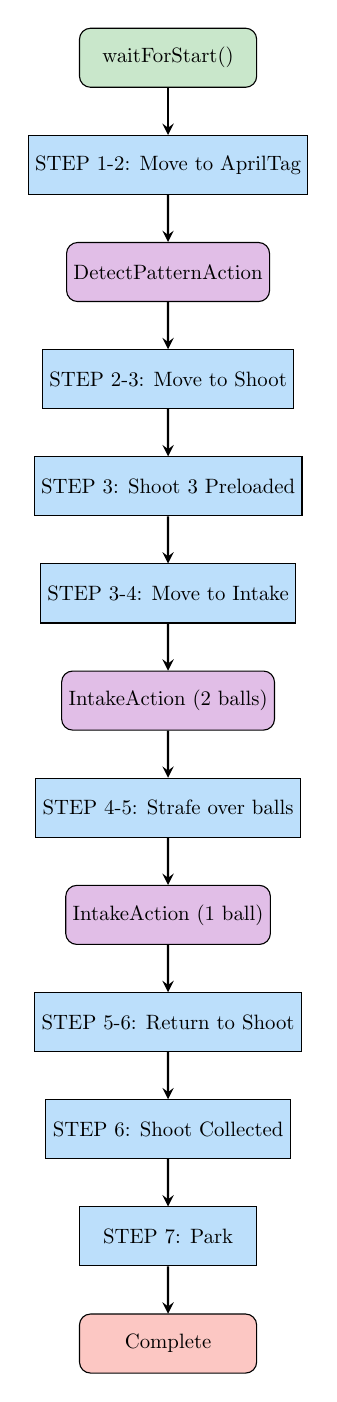
\begin{tikzpicture}[node distance=0.8cm, scale=0.75, transform shape]

% Nodes
\node (start) [startstop] {waitForStart()};
\node (step1) [process, below=of start] {STEP 1-2: Move to AprilTag};
\node (detect) [action, below=of step1] {DetectPatternAction};
\node (step2) [process, below=of detect] {STEP 2-3: Move to Shoot};
\node (step3) [process, below=of step2] {STEP 3: Shoot 3 Preloaded};
\node (step4a) [process, below=of step3] {STEP 3-4: Move to Intake};
\node (step4b) [action, below=of step4a] {IntakeAction (2 balls)};
\node (step5a) [process, below=of step4b] {STEP 4-5: Strafe over balls};
\node (step5b) [action, below=of step5a] {IntakeAction (1 ball)};
\node (step6a) [process, below=of step5b] {STEP 5-6: Return to Shoot};
\node (step6b) [process, below=of step6a] {STEP 6: Shoot Collected};
\node (step7) [process, below=of step6b] {STEP 7: Park};
\node (end) [startstop, below=of step7, fill=endcolor!30] {Complete};

% Arrows
\draw [arrow] (start) -- (step1);
\draw [arrow] (step1) -- (detect);
\draw [arrow] (detect) -- (step2);
\draw [arrow] (step2) -- (step3);
\draw [arrow] (step3) -- (step4a);
\draw [arrow] (step4a) -- (step4b);
\draw [arrow] (step4b) -- (step5a);
\draw [arrow] (step5a) -- (step5b);
\draw [arrow] (step5b) -- (step6a);
\draw [arrow] (step6a) -- (step6b);
\draw [arrow] (step6b) -- (step7);
\draw [arrow] (step7) -- (end);

\end{tikzpicture}
\end{center}

\textbf{ISSUE IDENTIFIED:} Steps 3-4 and 4-5 run intake \textit{after} movement completes (sequential). If the robot displaces during movement, the intake position may be wrong.

\newpage
% ============================================================================
\section{Shooting Sequence (Direct Control)}
% ============================================================================

\begin{center}
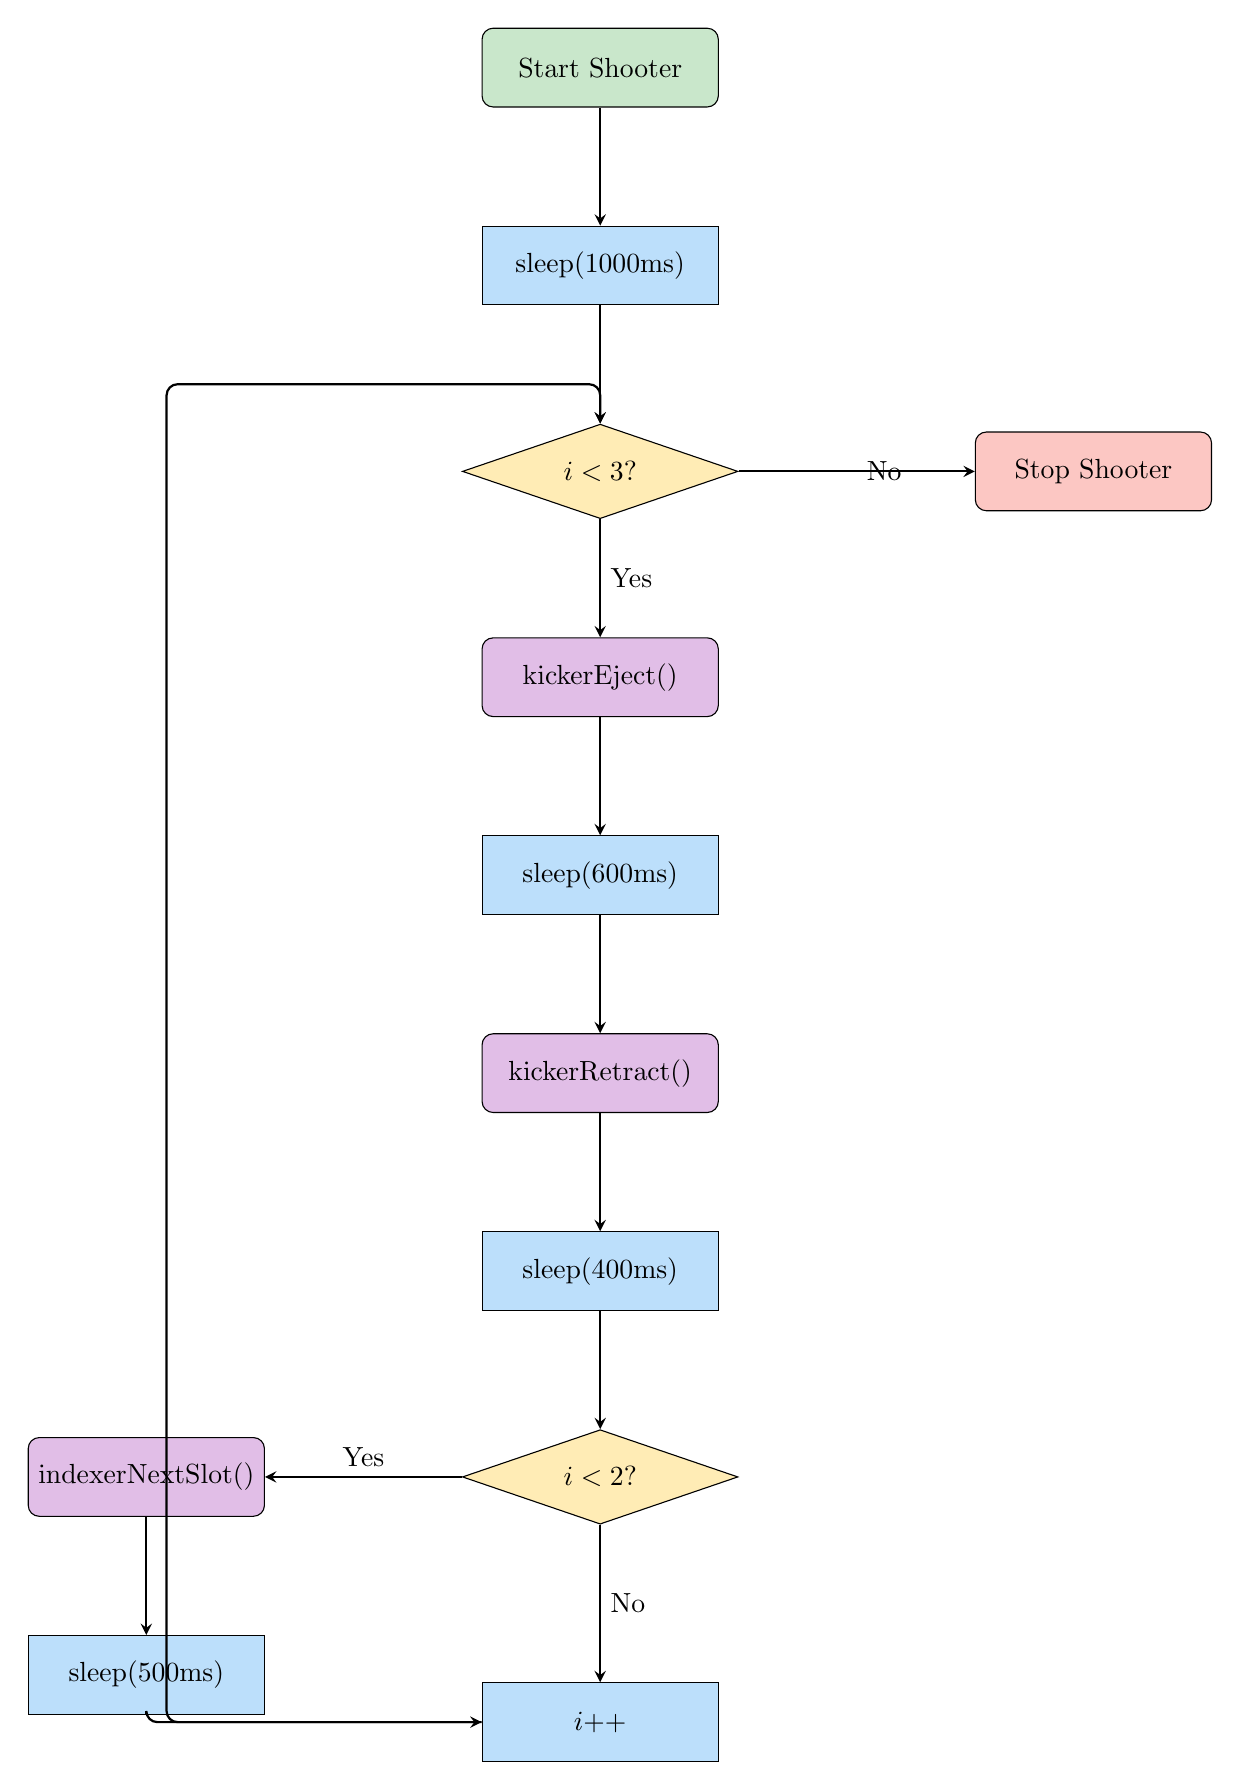
\begin{tikzpicture}[node distance=1.5cm, auto]

% Main Spine (Vertical)
\node (start) [startstop] {Start Shooter};
\node (spinup) [process, below=of start] {sleep(1000ms)};
\node (loop) [decision, below=of spinup] {$i < 3$?};
\node (kick) [action, below=of loop] {kickerEject()};
\node (wait1) [process, below=of kick] {sleep(600ms)};
\node (retract) [action, below=of wait1] {kickerRetract()};
\node (wait2) [process, below=of retract] {sleep(400ms)};

% Branching for Indexer
\node (check) [decision, below=of wait2] {$i < 2$?};
\node (index) [action, left=2.5cm of check] {indexerNextSlot()};
\node (wait3) [process, below=of index] {sleep(500ms)};

% Increment and Return
\node (inc) [process, below=2cm of check] {$i$++};
\node (stop) [startstop, right=3cm of loop, fill=endcolor!30] {Stop Shooter};

% Arrows and Routing
\draw [arrow] (start) -- (spinup);
\draw [arrow] (spinup) -- (loop);

% Loop Logic
\draw [arrow] (loop) -- node[right] {No} (stop);
\draw [arrow] (loop) -- node[right] {Yes} (kick);
\draw [arrow] (kick) -- (wait1);
\draw [arrow] (wait1) -- (retract);
\draw [arrow] (retract) -- (wait2);
\draw [arrow] (wait2) -- (check);

% Index Branch
\draw [arrow] (check) -- node[above] {Yes} (index);
\draw [arrow] (index) -- (wait3);
\draw [arrow] (wait3) |- (inc);   % Merge back to increment
\draw [arrow] (check) -- node[right] {No} (inc);

% Loop Return Path (LEFT SIDE)
% From 'inc' go left, up past everything, back to top of loop
\draw [arrow] (inc.west) -- ++(-4,0) |- ($(loop.north)+(0,0.5)$) -- (loop.north);

\end{tikzpicture}
\end{center}

\newpage
% ============================================================================
\section{IntakeWithIndexingAction State Machine}
% ============================================================================

This is the 3-phase state machine used during ground ball collection:

\begin{center}
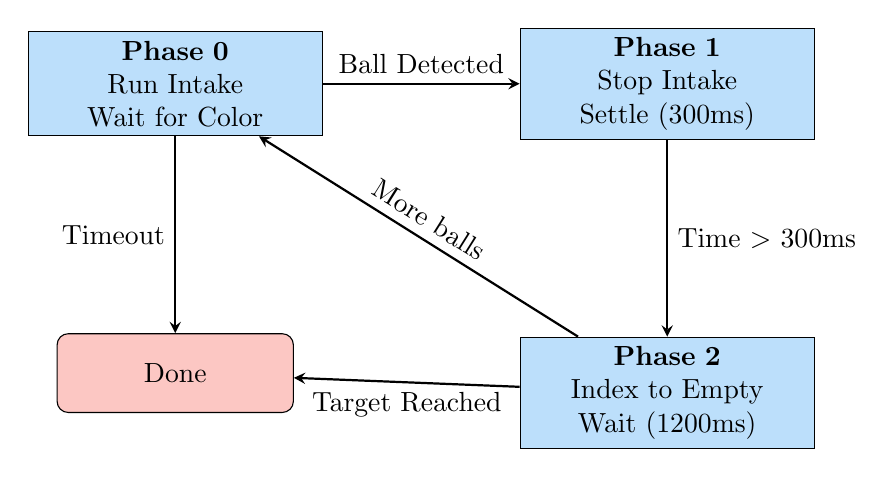
\begin{tikzpicture}[node distance=2.5cm, auto]

% Nodes laid out in a triangle
\node (phase0) [process, text width=3.5cm] {\textbf{Phase 0}\\Run Intake\\Wait for Color};
\node (phase1) [process, text width=3.5cm, right=of phase0] {\textbf{Phase 1}\\Stop Intake\\Settle (300ms)};
\node (phase2) [process, text width=3.5cm, below=of phase1] {\textbf{Phase 2}\\Index to Empty\\Wait (1200ms)};
\node (done) [startstop, below=of phase0, fill=endcolor!30] {Done};

% Arrows
\draw [arrow] (phase0) -- node[above] {Ball Detected} (phase1);
\draw [arrow] (phase1) -- node[right] {Time $>$ 300ms} (phase2);

% Return path from Phase 2 to Phase 0 (Diagonal up-left)
\draw [arrow] (phase2) -- node[above, sloped] {More balls} (phase0);

% Done conditions
\draw [arrow] (phase0) -- node[left] {Timeout} (done);
\draw [arrow] (phase2) -- node[below] {Target Reached} (done);

\end{tikzpicture}
\end{center}

\subsection{Known Issues}
\begin{enumerate}
    \item \textbf{Intake not starting}: The intake motor is only powered in Phase 0. If the action starts in wrong phase, intake won't run.
    \item \textbf{Synchronization}: The action runs \textit{after} movement completes, meaning robot is stationary during intake.
    \item \textbf{Color sensor reliability}: If sensor doesn't detect ball, action times out after 5 seconds.
\end{enumerate}

\newpage
% ============================================================================
\section{RevolverSubsystem State Machine}
% ============================================================================

\textbf{Note:} DecodeShootingAuto v4.0 \textit{bypasses} this state machine and uses direct control methods. However, understanding it helps debug issues.

\begin{center}
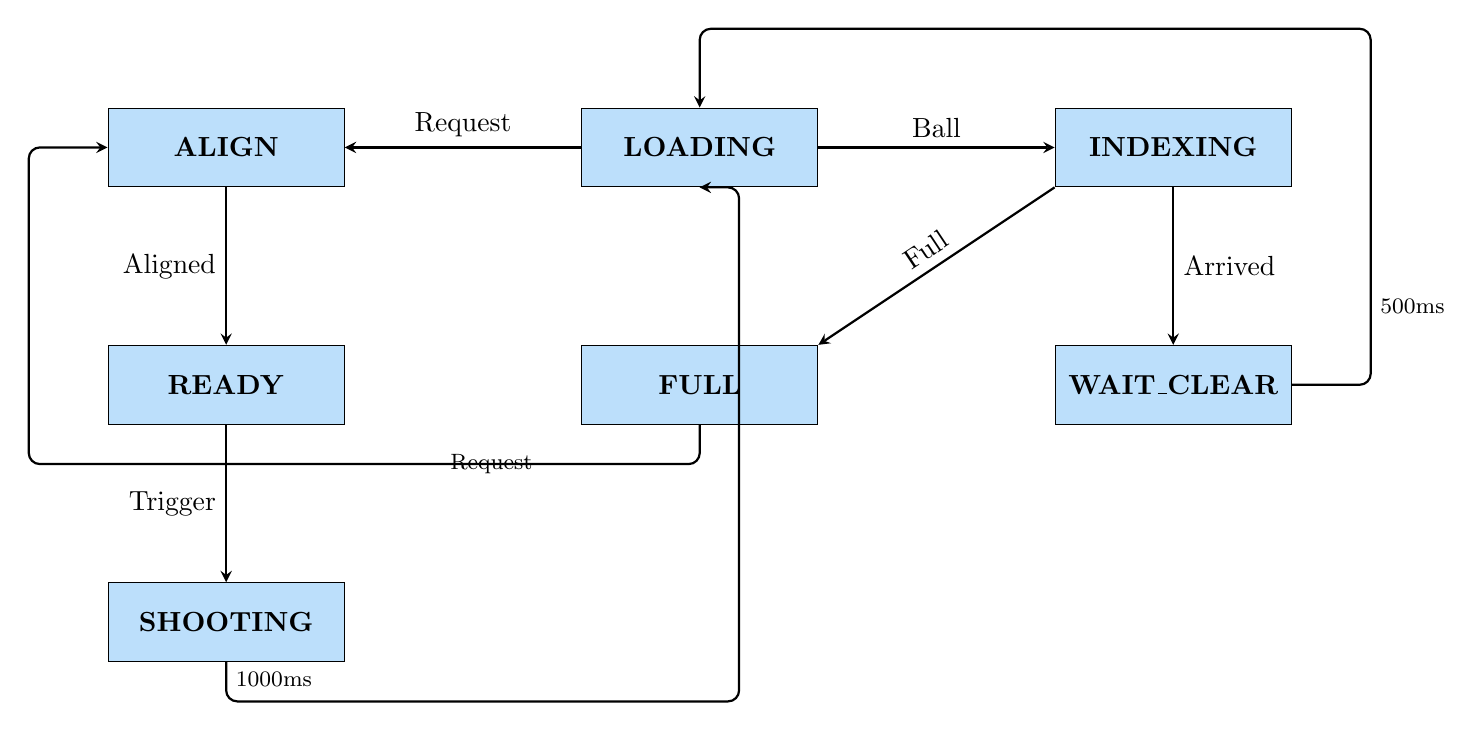
\begin{tikzpicture}[node distance=2cm, auto]

% Setup Columns with wide spacing
\node (loading) [process] {\textbf{LOADING}}; % Center (0,0)

% Right Column (Intake)
\node (indexing) [process, right=3cm of loading] {\textbf{INDEXING}};
\node (wait) [process, below=2cm of indexing] {\textbf{WAIT\_CLEAR}};

% Center Bottom
\node (full) [process, below=2cm of loading] {\textbf{FULL}};

% Left Column (Shooting)
\node (align) [process, left=3cm of loading] {\textbf{ALIGN}};
\node (ready) [process, below=2cm of align] {\textbf{READY}};
\node (shooting) [process, below=2cm of ready] {\textbf{SHOOTING}};

% --- Transitions with Explicit Routing ---

% 1. Loading -> Indexing (Straight)
\draw [arrow] (loading) -- node[above] {Ball} (indexing);

% 2. Indexing -> Wait (Straight Down)
\draw [arrow] (indexing) -- node[right] {Arrived} (wait);

% 3. Wait -> Loading (Wide Right & Top Loop to avoid Full/Indexing)
\draw [arrow] (wait.east) -- ++(1,0) |- ([yshift=1cm]loading.north) -- (loading.north);
\node [right, font=\footnotesize] at ($(wait.east)+(1,1)$) {500ms};

% 4. Indexing -> Full (Diagonal, clear of center)
\draw [arrow] (indexing.south west) -- node[sloped, above] {Full} (full.north east);

% 5. Loading -> Align (Straight)
\draw [arrow] (loading) -- node[above] {Request} (align);

% 6. Full -> Align (Wide Left Loop to avoid Ready)
\draw [arrow] (full.south) -- ++(0,-0.5) -| ([xshift=-1cm]align.west) -- (align.west);
\node [left, font=\footnotesize] at ($(full.south)+(-2,-0.5)$) {Request};

% 7. Align -> Ready (Straight Down)
\draw [arrow] (align) -- node[left] {Aligned} (ready);

% 8. Ready -> Shooting (Straight Down)
\draw [arrow] (ready) -- node[left] {Trigger} (shooting);

% 9. Shooting -> Loading (Wide Bottom Loop)
\draw [arrow] (shooting.south) -- ++(0,-0.5) -| ([xshift=0.5cm]loading.south) -- (loading.south);
\node [below right, font=\footnotesize] at (shooting.south) {1000ms};

\end{tikzpicture}
\end{center}

\subsection{State Descriptions}
\begin{description}
    \item[LOADING] Empty slot at intake position, waiting for ball
    \item[INDEXING] Moving indexer to next empty slot
    \item[WAIT\_FOR\_INTAKE\_CLEAR] Pause after indexing (500ms)
    \item[FULL] All 3 slots filled
    \item[SHOOTING\_ALIGN] Rotating target slot to shooter position (240°)
    \item[READY\_TO\_SHOOT] Aligned, waiting for manual trigger
    \item[SHOOTING] Kicker sequence active
\end{description}

\newpage
% ============================================================================
\section{Color Detection Logic}
% ============================================================================

\begin{center}
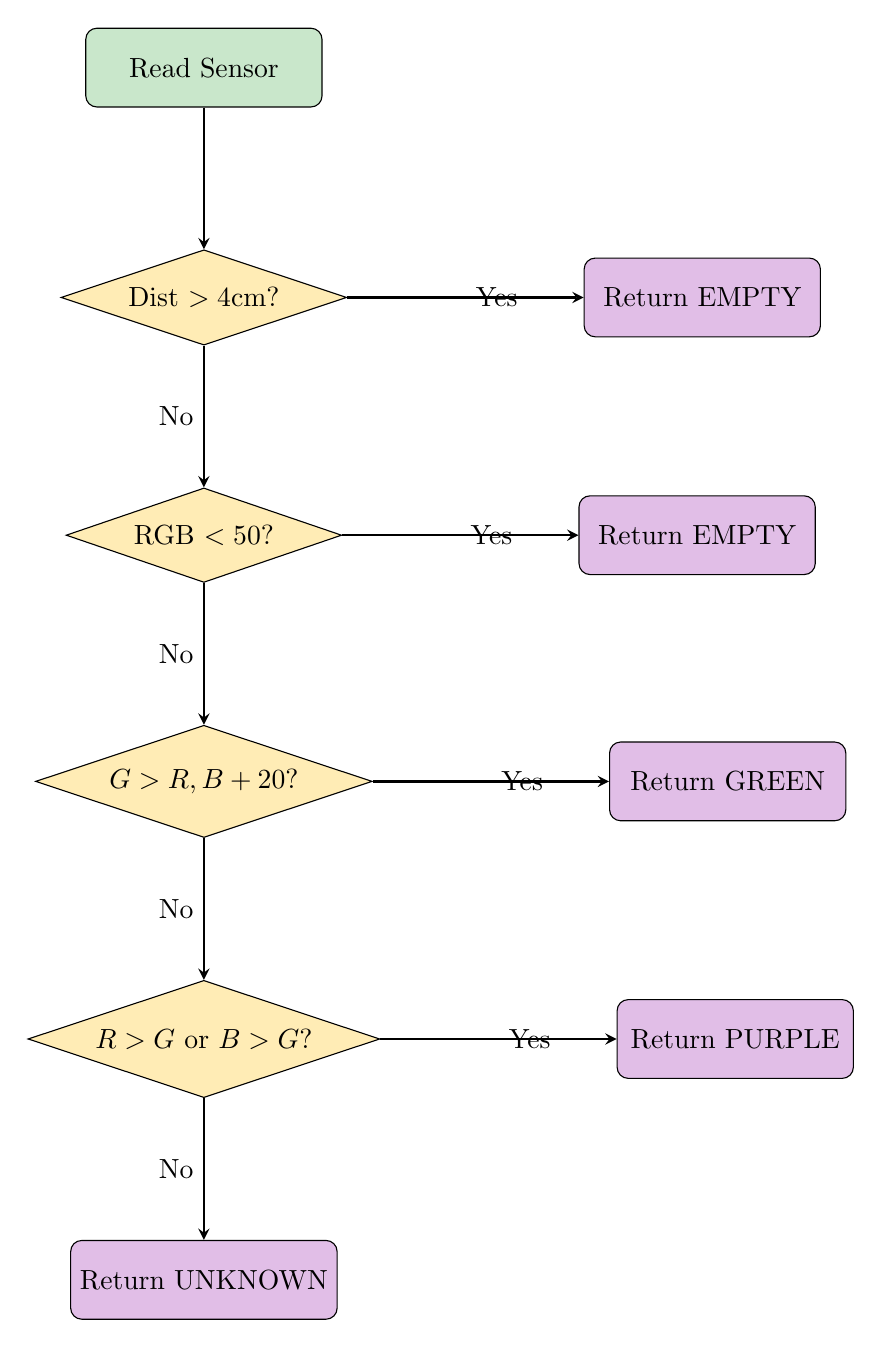
\begin{tikzpicture}[node distance=1.8cm, auto]

% Main Spine (Vertical)
\node (start) [startstop] {Read Sensor};
\node (dist) [decision, below=of start] {Dist $> 4$cm?};
\node (rgb) [decision, below=of dist] {RGB $< 50$?};
\node (green) [decision, below=of rgb] {$G > R,B+20$?};
\node (purple) [decision, below=of green] {$R>G$ or $B>G$?};
\node (unknown) [action, below=of purple] {Return UNKNOWN};

% Results (Right side)
\node (empty1) [action, right=3cm of dist] {Return EMPTY};
% Shared node for second empty condition for cleaner graph
\node (empty2) [action, right=3cm of rgb] {Return EMPTY}; 
\node (gret) [action, right=3cm of green] {Return GREEN};
\node (pret) [action, right=3cm of purple] {Return PURPLE};

% Arrows
\draw [arrow] (start) -- (dist);

% Distance Check
\draw [arrow] (dist) -- node[right] {Yes} (empty1);
\draw [arrow] (dist) -- node[left] {No} (rgb);

% Darkness Check
\draw [arrow] (rgb) -- node[right] {Yes} (empty2);
\draw [arrow] (rgb) -- node[left] {No} (green);

% Green Check
\draw [arrow] (green) -- node[right] {Yes} (gret);
\draw [arrow] (green) -- node[left] {No} (purple);

% Purple Check
\draw [arrow] (purple) -- node[right] {Yes} (pret);
\draw [arrow] (purple) -- node[left] {No} (unknown);

\end{tikzpicture}
\end{center}

\newpage
% ============================================================================
\section{Trajectory Waypoints}
% ============================================================================

\begin{center}
\begin{tabular}{|c|c|c|c|l|}
\hline
\textbf{Step} & \textbf{X} & \textbf{Y} & \textbf{Heading} & \textbf{Purpose} \\
\hline
Start & -61 & -35 & 0° & Starting position \\
AprilTag & -37 & -13 & 160° & Read randomization pattern \\
Shoot 1 & -35 & -31 & 230° & Shoot preloaded (backed up) \\
Intake 1 & -11 & -30 & 270° & First intake position \\
Intake 2 & -11 & -55 & 270° & Strafe over balls \\
Shoot 2 & -35 & -31 & 230° & Shoot collected \\
Park & -5 & -53 & 90° & Final parking \\
\hline
\end{tabular}
\end{center}

\section{Debugging Checklist}

\begin{enumerate}
    \item \textbf{Intake not spinning?}
    \begin{itemize}
        \item Check \texttt{setIntakePowerDirect()} is called in Phase 0
        \item Verify \texttt{INTAKE\_POWER = 1.0}
        \item Check motor configuration in RevolverSubsystem constructor
    \end{itemize}
    
    \item \textbf{Ball not detected?}
    \begin{itemize}
        \item Check color sensor distance threshold (4cm)
        \item Verify RGB thresholds for GREEN/PURPLE detection
        \item Add telemetry for \texttt{getCurrentColor()} and \texttt{getDistance()}
    \end{itemize}
    
    \item \textbf{Indexer not rotating?}
    \begin{itemize}
        \item Verify \texttt{indexerNextSlot()} is called
        \item Check \texttt{TICKS\_PER\_SLOT = 96}
        \item Verify \texttt{isIndexerAtTarget()} returns correctly
    \end{itemize}
\end{enumerate}



% ============================================================================
\section{Future Work (Tomorrow's Checklist)}
% ============================================================================

\begin{enumerate}
    \item \textbf{Increase Shooting Power}
    \begin{itemize}
        \item Optimize power level for range and speed (target > 0.5).
        \item Verify trajectory with higher power.
    \end{itemize}

    \item \textbf{Create Red Team Version}
    \begin{itemize}
        \item Duplicate autonomous for Red Alliance.
        \item Mirror coordinates (Y axis inversion).
        \item Adjust heading targets.
    \end{itemize}

    \item \textbf{Correct Intake Speed}
    \begin{itemize}
        \item Tune \texttt{moveSpeed} in \texttt{SmartIntakeAction}.
        \item Verify intake motor power efficiency.
        \item Ensure synchronization with robot velocity.
    \end{itemize}

    \item \textbf{Correct Distance Moved}
    \begin{itemize}
        \item Calibrate \texttt{endY} coordinate in \texttt{SmartIntakeAction}.
        \item Verify "Travel Distance" vs "Intake Distance".
        \item Adjust \texttt{TIMEOUT\_MS} if distance changes.
    \end{itemize}
\end{enumerate}

\end{document}
